\documentclass[size=14pt,paper=screen,style=paintings]{powerdot}
\usepackage{mathtext}
\usepackage[T2A]{fontenc}
\usepackage[utf8]{inputenc}
\usepackage[russian]{babel}
\usepackage{indentfirst}
\usepackage[intlimits]{amsmath}
\usepackage{lscape}
\usepackage{amssymb}
\usepackage{tabularx}
\usepackage{setspace}
\usepackage{graphicx}
\graphicspath{{images/}}
\DeclareGraphicsExtensions{.pdf,.png,.jpg, .eps}

\title{\vspace*{-1cm}{\large Компьютерная игра 'The Snake'}}
\author{\noindent Дегтярев Максим Эдуардович  
\and Научный руководитель: \and доцент кафедры 813
 Мокряков  \and Алексей Викторович}

\begin{document}

\maketitle

%------------------------------------------------------%

\begin{slide}{{\normalsize Цели работы}}

Основная цель данной работы - получить работоспособную реализацию компьютерной игры 'The Snake', дополненной различными функциями, которые отсутствуют в оригинальной версии игры.
\begin{center}
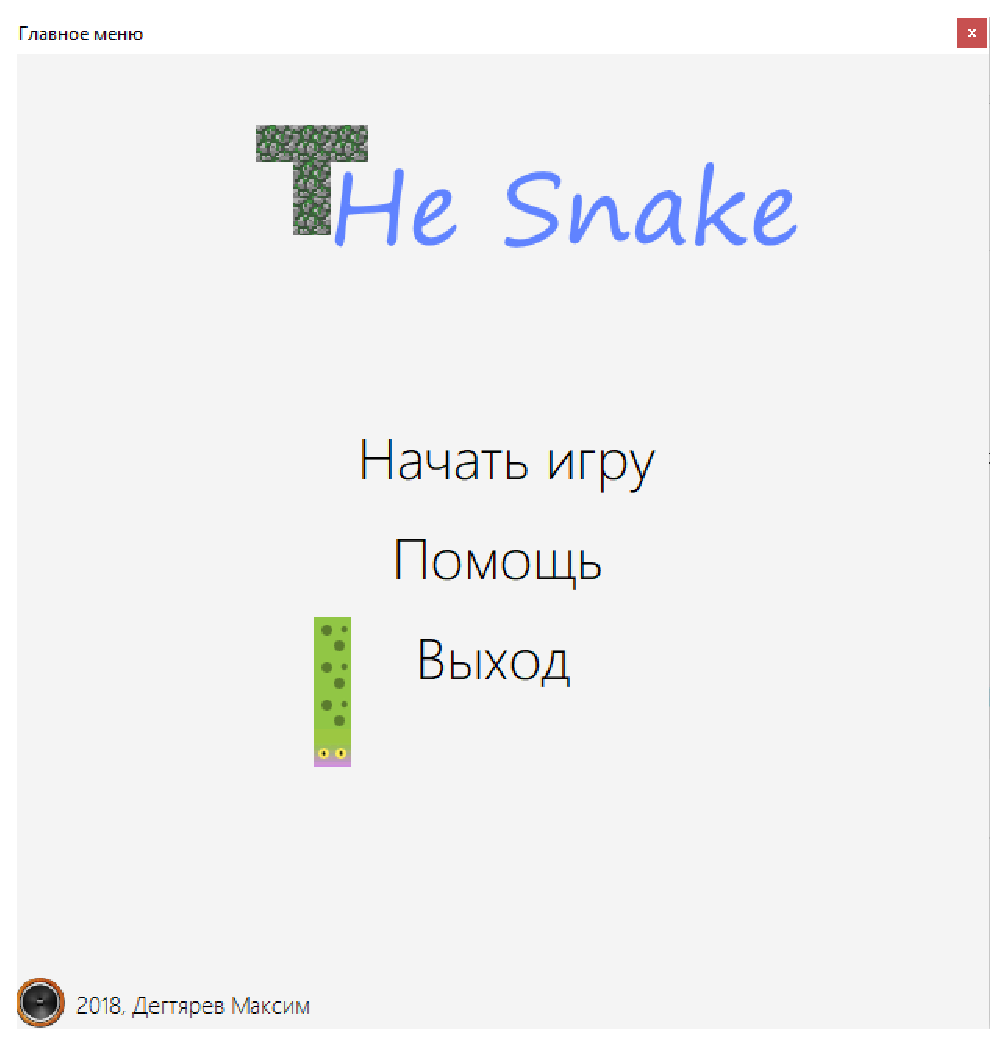
\includegraphics[scale=0.3]{img2.eps}
\end{center}
\end{slide}

\begin{slide}{{\normalsize Задачи}}
\begin{enumerate}
\vspace*{1cm}
\item Создать основной класс
\item Создать текстуры
\item Реализовать управление и механику игры
\item Сделать горячие клавиши
\item Реализовать редактор карт
\item Реализовать ИУ
\item Написать инструкцию к игре
\end{enumerate}
\end{slide}
%--------------------------------------------------------------------

%--------------------------------------------------------------------

\begin{slide}{{\normalsize Результат}}
\vspace*{1cm}
В результате была получена рабочая реализация компьютерной игры 'The Snake' с возможность создавать и редактировать карты, задавать в редакторе режим игры, цель. Компьютерная игра выполнена в приятной для глаз цветовой схеме.
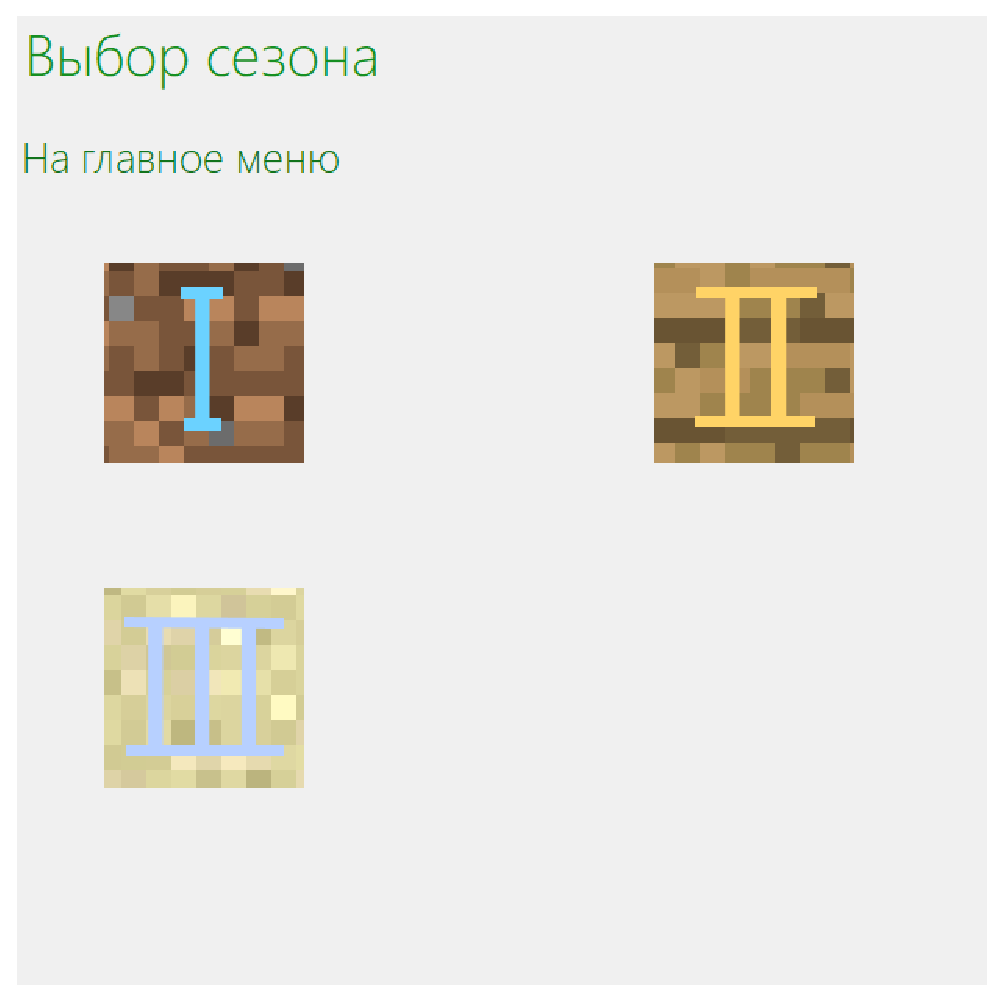
\includegraphics[scale=0.3]{img3.eps}

\end{slide}

\begin{slide}{{\normalsize Результат}}
\vspace*{1cm}
\begin{center}
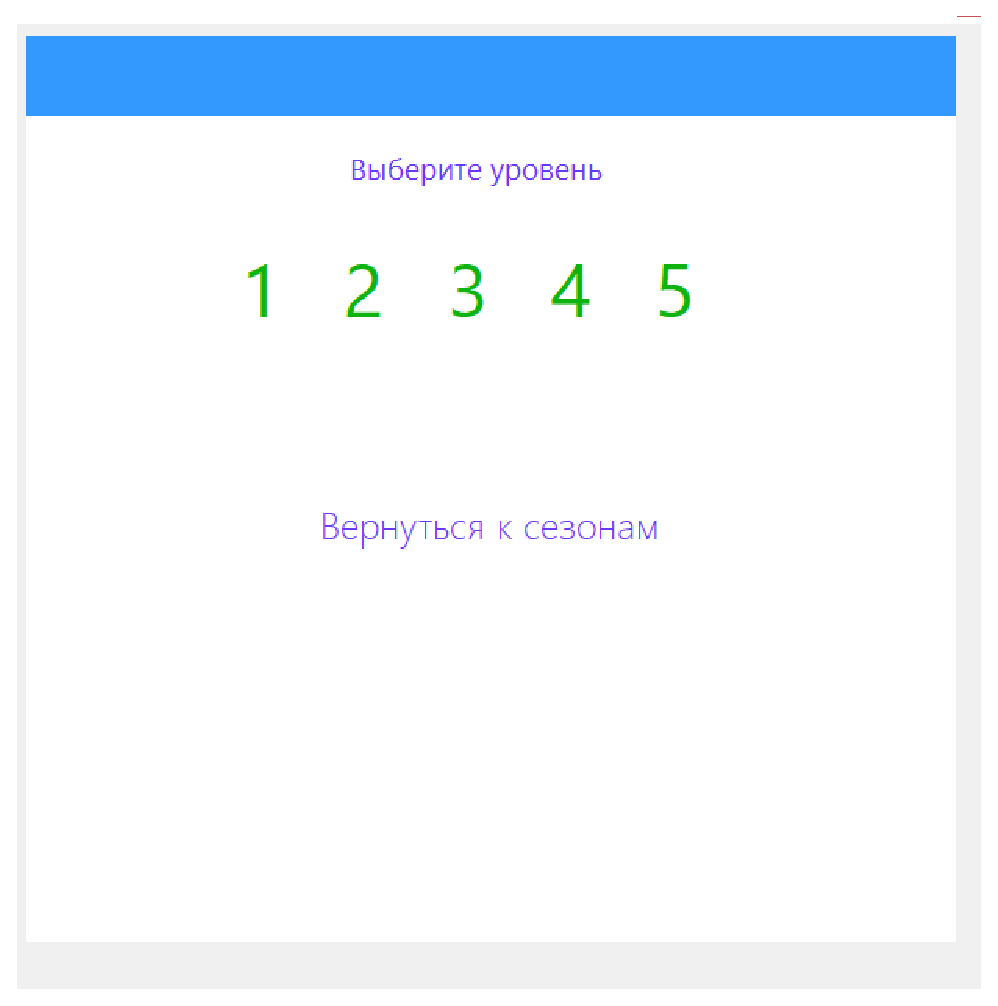
\includegraphics[scale=0.3]{img4.eps}
\end{center}
\end{slide}

\begin{slide}{{\normalsize Результат}}
\vspace*{1cm}
\begin{center}
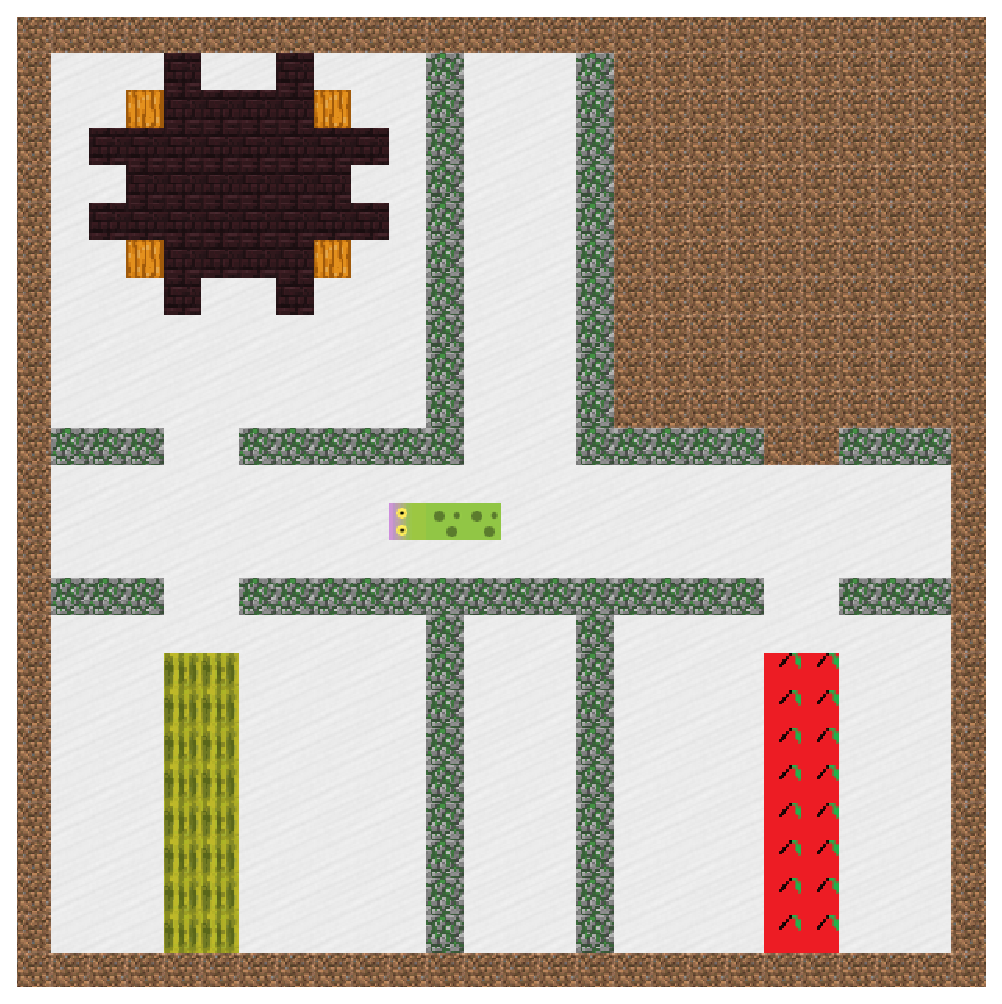
\includegraphics[scale=0.3]{img8.eps}
\end{center}
\end{slide}

\begin{slide}{{\normalsize Результат}}
\vspace*{1cm}
\begin{center}
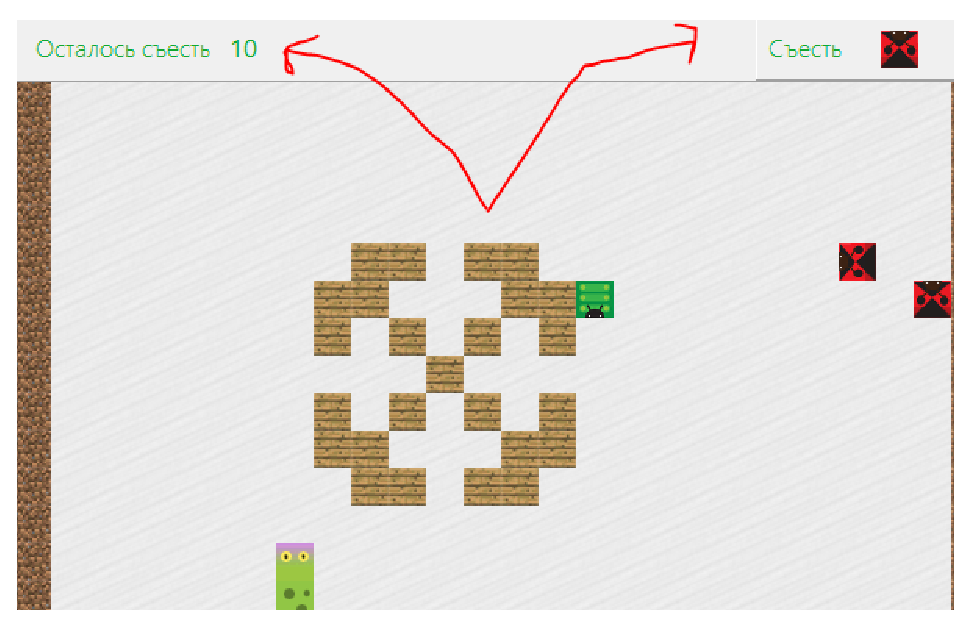
\includegraphics[scale=0.3]{img9.eps}
\end{center}

\end{slide}

\begin{slide}{{\normalsize Результат}}
\vspace*{1cm}
\begin{center}
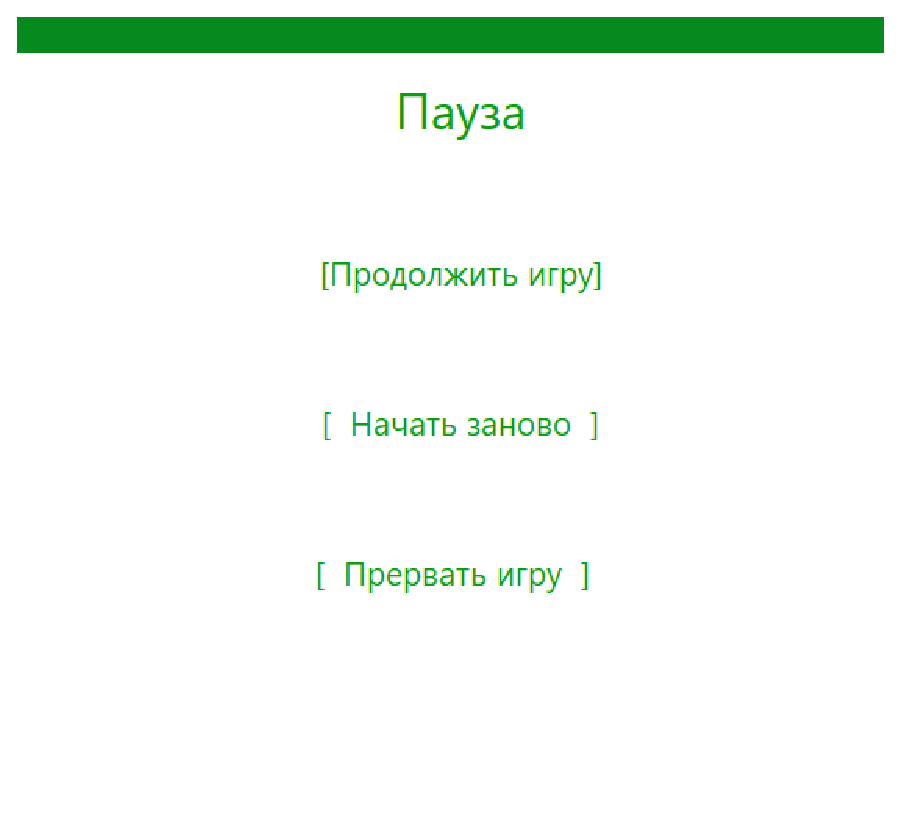
\includegraphics[scale=0.5]{img10.eps}
\end{center}
\end{slide}

\begin{slide}{{\normalsize Результат}}
\vspace*{1cm}
\begin{center}
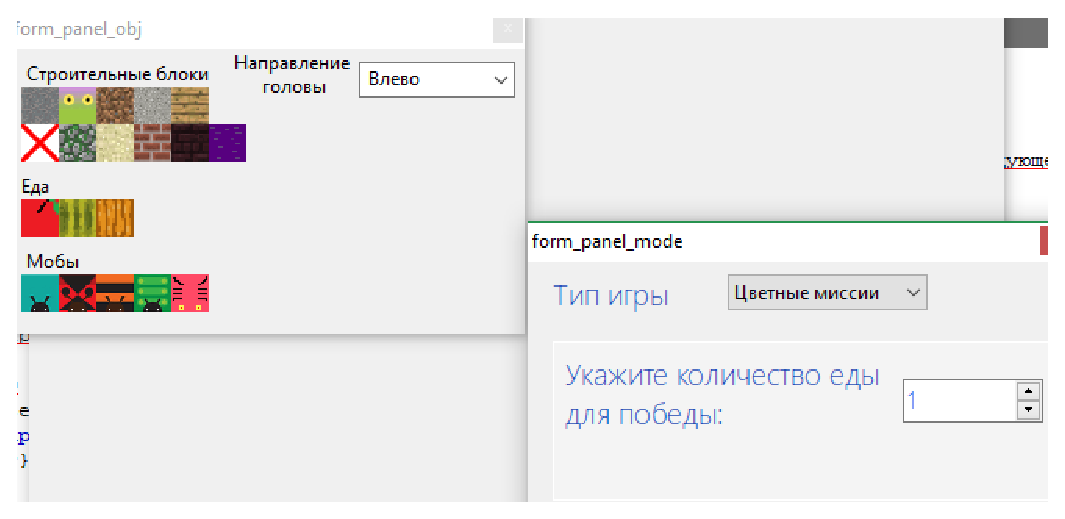
\includegraphics[scale=0.5]{img15.eps}
\end{center}

\end{slide}
\end{document}



